\chapter{Selbstüberwachtes Lernen}
\label{chap:selfsupervised}
\qq{Warum besteht interesse an unsupervised/selfsupervised Lernen?}
\citeauthor*{SunRevisitingUnreasonableEffectiveness2017} stellen fest, dass ein Teil des Erfolges von CNNs auf
die Verfügbarkeit von großen annotierten Datensets wie ImageNet zurückzuführen ist. 
Jedoch ist die Anzahl der Bilder im ImageNet-Datenset in den vergangen Jahren gleich geblieben, während die  verfügbare Netzwerkkapazität und GPU-Rechenleistung angestiegen ist.
\citeauthor{SunRevisitingUnreasonableEffectiveness2017} zeigen mithilfe des JFT-300M-Datensets (300 Millionen annotierte Bilder), dass die Performanz von allen getesteten Aufgaben (Klassifizerung, Segmentierung, etc.)
logaritmisch zur Datenmenge ansteigt. 

Für eine linearen Anstieg in Performanz bräuchte man eine exponetiell mehr Daten.
Die annotierung von Datensets ist immer ein teuerer Prozess \autocite[988]{ValvenyDatasetsAnnotationsDocument2014}.
Die die manuelle Annotation einer Dokumentenseite mehr als eine Stunde in Anspruch nehmen. 

% Das kollaborative Annotieren von Datensets ermöglicht es große Datenmengen in hoher Qualität zu annotieren.
% Das reCAPTCHA-Projekt \cite{reCAPTCHA} h  
% semiautomatisch



\begin{figure}[htbp!]
    \centering
    \caption{Schematische Darstellung von ML-Methoden}
    \label{fig:all}
    \subfloat[Neuronales Netzwerke und Training \cite{CholletDeeplearningPython2018}\label{fig:sub1}]{    
      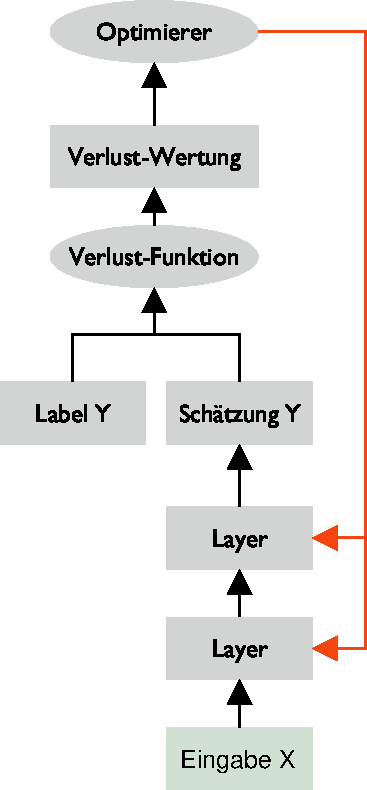
\includegraphics[width=0.3\textwidth, valign=t]{figures/graphs/chollet2018supervised.pdf}
      \vphantom{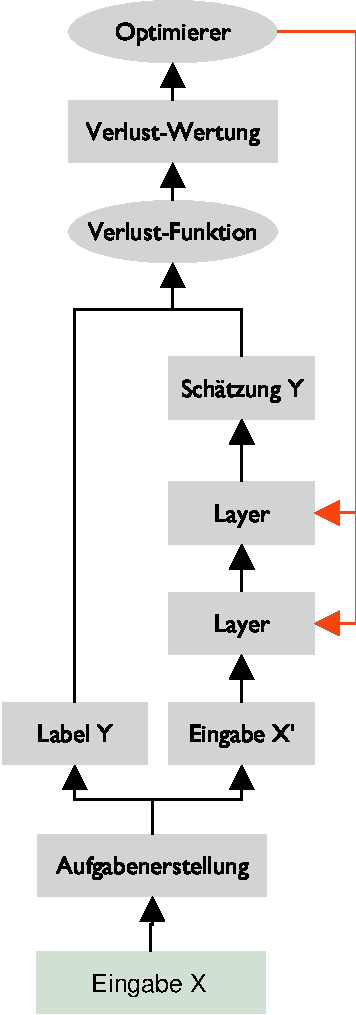
\includegraphics[width=0.3\textwidth,valign=t]{figures/graphs/selfsupervised.pdf}}
    }
    \subfloat[Autoencoder\label{fig:sub2}]{    
      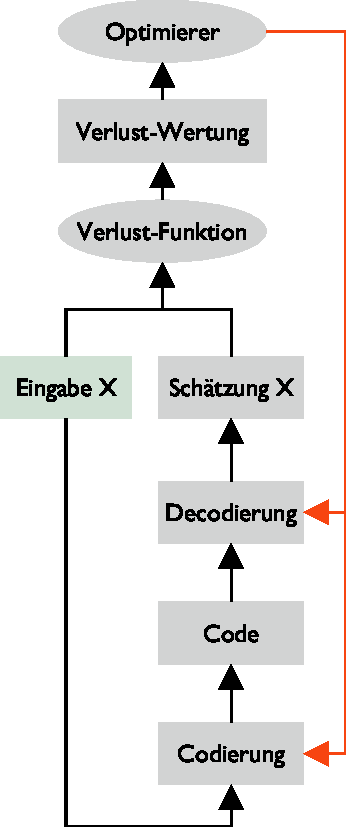
\includegraphics[width=0.3\textwidth, valign=t]{figures/graphs/autoencoder.pdf}
      \vphantom{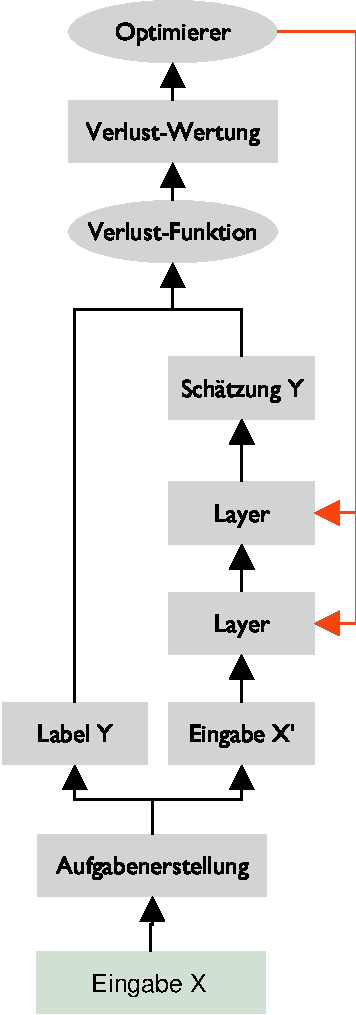
\includegraphics[width=0.3\textwidth,valign=t]{figures/graphs/selfsupervised.pdf}}
    }
    \subfloat[Selbstüberwachtes Lernen\label{fig:sub3}]{    
      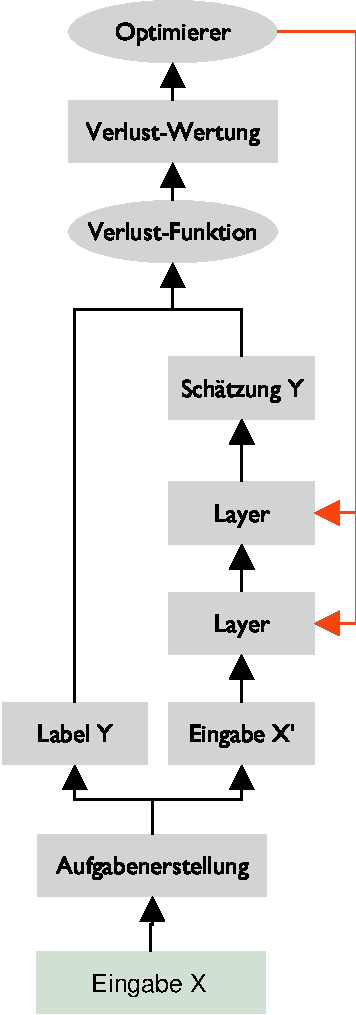
\includegraphics[width=0.3\textwidth, valign=t]{figures/graphs/selfsupervised.pdf}
    }
    
    
\end{figure}
\vspace{0.5cm}

\section{Unüberwachtes Lernen von unterscheidbaren Features}

\sfigure{Workflow}{figures/graphs/dosovitskiy2015_workflow.pdf}

Jigsaw
\cite{NorooziUnsupervisedLearningVisual2016}
% \begin{figure}
%     \includegraphics[]{figures/graphs/exp.pdf} 
%     \caption{Image}
%   \end{figure}
